\documentclass{beamer}
\usepackage{amsfonts,amsmath,oldgerm}
\usetheme{sintef}

\newcommand{\testcolor}[1]{\colorbox{#1}{\textcolor{#1}{test}}~\texttt{#1}}

\usefonttheme[onlymath]{serif}


% adicionar o numero na lista final da apresentação
\setbeamertemplate{bibliography item}{\insertbiblabel}

\newcommand{\hrefcol}[2]{\textcolor{cyan}{\href{#1}{#2}}}
\title{Desenvolvimento de um sistema de telemetria para veículos Formula SAE}
\course{Trabalho de conclusão de curso}
\author{Thalles Nonato Leal Santos}
\IDnumber{\href{mailto:eusouthalles@ic.ufrj.br}{eusouthalles@ic.ufrj.br}, \href{mailto:tnonato@cos.ufrj.br}{tnonato@cos.ufrj.br}}

\begin{document}
\maketitle

\section{Introdução}

\begin{frame}{Telemetria}
	\begin{itemize}
		
		 \item O termo \textbf{telemetria} tem origem no grego:
		\begin{itemize}
			\item \textit{tele} = distante
			\item \textit{metron} = medida
		\end{itemize}
		
		\item Assim, telemetria significa literalmente ``medição à distância''.
		
		
		\item A telemetria surgiu da necessidade de monitorar sistemas remotos ou de difícil acesso.
		
		
		\item Seu principal objetivo é coletar dados de sensores e transmiti-los para uma estação de análise em tempo real.
		
		\item Historicamente, foi utilizada em aplicações aeroespaciais, militares e aeronáuticas, principalmente no monitoramento de foguetes, mísseis e aeronaves.
		

	\end{itemize}
\end{frame}

\begin{frame}{Telemetria no Automobilismo}
	\begin{itemize}
		\item A utilização da telemetria no automobilismo teve início nas categorias de alto desempenho, principalmente na Fórmula 1, durante as décadas de 1970 e 1980.
		
		\item Inicialmente, os sistemas eram utilizados apenas para aquisição de dados após testes e corridas, por meio de registradores embarcados (dataloggers).

		\item Na década de 1990, a transmissão de dados em tempo real entre o carro e os boxes tornou-se uma grande evolução tecnológica nas competições.
		
		\item A telemetria passou então a ser utilizada como ferramenta estratégica para análise de desempenho, ajustes na configuração do carro e diagnóstico de falhas durante as provas.
	\end{itemize}
\end{frame}


\begin{frame}[fragile]{Telemetria}
	
	\begin{columns}[c]
		
		% IMAGEM
		\column{0.45\textwidth}
		\centering
		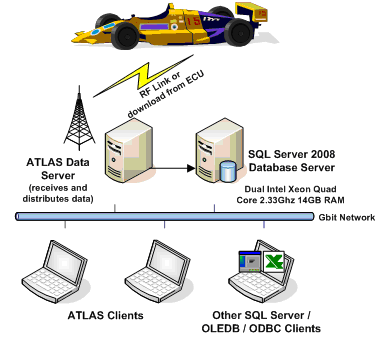
\includegraphics[height=5cm,keepaspectratio]{assets/ecu_atlas_client.png}
		
		\small Sistema de telemetria
		
		% TEXTO
		\column{0.55\textwidth}
		
		\begin{itemize}
			\item Sensores capturam dados do carro
			\item Dados são centralizados em um módulo principal (ECU)
			\item Parte dos dados é transmitida em tempo real via rádio frequência (RF)
			\item O sinal RF é enviado por antenas transmissoras e captado por antenas receptoras na equipe
			\item O restante é armazenado para análise posterior
		\end{itemize}
		
	\end{columns}
	
\end{frame}

\begin{frame}[fragile]{Telemetria}
	\begin{center}
		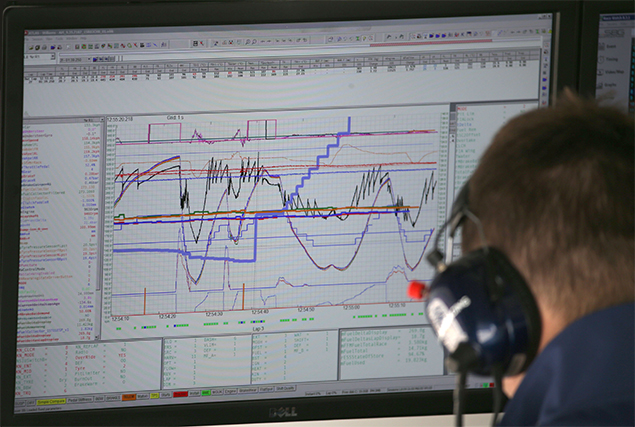
\includegraphics[width=0.5\textwidth]{assets/F1-telemetria.jpg}
	\end{center}
\end{frame}

\begin{frame}[fragile]{Equipe Icarus UFRJ de Formula SAE}
To set a typical title page, you call some commands in the preamble:
\begin{block}{The Commands for the Title Page}
\begin{verbatim}
\title{Sample Title}
\subtitle{Sample subtitle}
\author{First Author, Second Author}
\date{\today} % Can also be (ab)used for conference name &c.
\end{verbatim}
\end{block}
You can then write out the title page with \verb|\maketitle|.

To set a \textbf{background image} use the \verb|\titlebackground| command 
before \verb|\maketitle|; its only argument is the name (or path) of a graphic 
file.

If you use the \textbf{starred version} \verb|\titlebackground*|, the image 
will be clipped to a split view on the right side of the title slide.

\end{frame}

\begin{frame}[fragile]{Writing a Simple Slide}
\framesubtitle{It's really easy!}
\begin{itemize}[<+->]
\item A typical slide has bulleted lists
\item These can be uncovered in sequence
\end{itemize}
\begin{block}{Code for a Page with an Itemised List}<+->
\begin{verbatim}
\begin{frame}{Writing a Simple Slide}
  \framesubtitle{It's really easy!}
  \begin{itemize}[<+->]
    \item A typical slide has bulleted lists
    \item These can be uncovered in sequence
  \end{itemize}\end{frame}
\end{verbatim}
\end{block}
\end{frame}

\section{Revisão Teórica}

\footlinecolor{sintefyellow}
\begin{frame}[fragile]{Changing Slide Style}
\begin{itemize}
\item You can select the white or \textit{maincolor} \textbf{slide style} \emph{in the 
preamble} with \verb|\themecolor{white}| (default) or \verb|\themecolor{main}|
      \begin{itemize}
      \item You should \emph{not} change these within the document: Beamer does 
      not like it
      \item If you \emph{really} must, you may have to add 
      \verb|\usebeamercolor[fg]{normal text}| in the slide
      \end{itemize}
\item You can change the \textbf{footline colour} with 
\verb|\footlinecolor{color}|
      \begin{itemize}
      \item Place the command \emph{before} a new \verb|frame|
      \item There are four ``official'' colors: 
      \testcolor{maincolor}, \testcolor{sintefyellow}, 
      \testcolor{sintefgreen}, \testcolor{sintefdarkgreen}
      \item Default is no footline; you can restore it with 
      \verb|\footlinecolor{}|
      \item Others may work, but no guarantees!
      \item Should \emph{not} be used with the \verb|maincolor| theme!
      \end{itemize}
\end{itemize}
\end{frame}

\begin{frame}[fragile]{Blocks}
\begin{columns}
\begin{column}{0.3\textwidth}
\begin{block}{Standard Blocks}
These have a color coordinated with the footline (and grey in the blue theme)
\begin{verbatim}
\begin{block}{title}
content...
\end{block}
\end{verbatim}
\end{block}
\end{column}
\begin{column}{0.7\textwidth}
\begin{colorblock}[black]{sinteflightgreen}{Colour Blocks}
Similar to the ones on the left, but you pick the colour. Text will be white by 
default, but you may set it with an optional argument.
\small
\begin{verbatim}
\begin{colorblock}[black]{sinteflightgreen}{title}
content...
\end{colorblock}
\end{verbatim}
\end{colorblock}
The ``official'' colours of colour blocks are: \testcolor{sinteflilla}, 
\testcolor{maincolor}, \testcolor{sintefdarkgreen}, and 
\testcolor{sintefyellow}.
\end{column}
\end{columns}
\end{frame}

\footlinecolor{}
\begin{frame}[fragile]{Using Colours}
\begin{itemize}[<alert@2>]
  \item You can use colours with the
        \verb|\textcolor{<color name>}{text}| command
  \item The colours are defined in the \texttt{sintefcolor} package:
  \begin{itemize}
  \item Primary colours: \testcolor{maincolor} and its sidekick 
  \testcolor{sintefgrey}
  \item Three shades of green: \testcolor{sinteflightgreen}, 
  \testcolor{sintefgreen}, \testcolor{sintefdarkgreen}
  \item Additional colours: \testcolor{sintefyellow}, \testcolor{sintefred}, 
        \testcolor{sinteflilla}
        \begin{itemize}
        \item These may be shaded---see the \verb|sintefcolor| documentation or 
        the \hrefcol{https://sintef.sharepoint.com/sites/stottetjenester/%
        kommunikasjon/grafisk-profil-new/Sider/default.aspx}{SINTEF profile 
        manual}
        \end{itemize}
  \end{itemize}
  \item Do \emph{not} abuse colours: \verb|\emph{}| is usually enough
  \item Use \verb|\alert{}| to bring the \alert<2->{focus} somewhere
  \item<2- | alert@2> If you highlight too much, you don't highlight at all!
\end{itemize}
\end{frame}

\begin{frame}[fragile]{Adding images}
\begin{columns}
\begin{column}{0.7\textwidth}
Adding images works like in normal \LaTeX:
\begin{block}{Code for Adding Images}
\begin{verbatim}
\usepackage{graphicx}
% ...

\includegraphics[width=\textwidth]
{assets/logo_RGB}
\end{verbatim}
\end{block}
\end{column}
\begin{column}{0.3\textwidth}

\includegraphics[width=\textwidth]
{assets/logo_RGB}
\end{column}
\end{columns}
\end{frame}

\begin{frame}[fragile]{Splitting in Columns}
Splitting the page is easy and common;
typically, one side has a picture and the other text:
\begin{columns}
\begin{column}{0.6\textwidth}
This is the first column
\end{column}
\begin{column}{0.3\textwidth}
And this the second
\end{column}
\end{columns}
\begin{block}{Column Code}
\begin{verbatim}
\begin{columns}
    \begin{column}{0.6\textwidth}
        This is the first column
    \end{column}
    \begin{column}{0.3\textwidth}
        And this the second
    \end{column}
    % There could be more!
\end{columns}
\end{verbatim}
\end{block}
\end{frame}

\begin{chapter}[assets/background_negative]{}{Special Slides}
\begin{itemize}
\item Chapter slides
\item Side-picture slides
\end{itemize}
\end{chapter}

\footlinecolor{sintefred}
\begin{frame}[fragile]{Chapter slides}
\begin{itemize}
\item Similar to \verb|frame|s, but with a few more options
\item Opened with \verb|\begin{chapter}[<image>]{<color>}{<title>}|
\item Image is optional, colour and title are mandatory
\item There are seven ``official'' colours: \testcolor{maincolor}, 
\testcolor{sintefdarkgreen}, \testcolor{sintefgreen}, 
\testcolor{sinteflightgreen}, \testcolor{sintefred}, \testcolor{sintefyellow}, 
\testcolor{sinteflilla}.
      \begin{itemize}
      \item Strangely enough, these are \emph{more} than the official colours 
      for the footline.
      \item It may still be a nice touch to change the footline of following 
      slides to the same color of a chapter slide. Your choice.
      \end{itemize}
\item Otherwise, \verb|chapter| behaves just like \verb|frame|.
\end{itemize}
\end{frame}

\begin{sidepic}{assets/background}{Side-Picture Slides}
\begin{itemize}
\item Opened with \texttt{$\backslash$begin\{sidepic\}\{<image>\}\{<title>\}}
\item Otherwise, \texttt{sidepic} works just like \texttt{frame}
\end{itemize}
\end{sidepic}

\footlinecolor{}
\begin{frame}
\frametitle{Fonts}
\begin{itemize}
\item The paramount task of fonts is being readable
\item There are good ones...
  \begin{itemize}
  \item {\textrm{Use serif fonts only with high-definition projectors}}
  \item {\textsf{Use sans-serif fonts otherwise (or if you simply prefer 
them)}}
  \end{itemize}
\item ... and not so good ones:
  \begin{itemize}
  \item {\texttt{Never use monospace for normal text}}
  \item {\frakfamily Gothic, calligraphic or weird fonts: should always: be
  avoided}
\end{itemize}
\end{itemize}
\end{frame}

\begin{frame}[fragile]{Look}
\begin{itemize}
\item To insert a final slide with the title and final thanks, use \verb|\backmatter|.
      \begin{itemize}
      \item The title also appears in footlines along with the author name, you can change this text with \verb|\footlinepayoff|
      \item You can remove the title from the final slide with \verb|\backmatter[notitle]|
      \end{itemize}
\item The aspect ratio defaults to 16:9, and you should not change it to 4:3
      for old projectors as it is inherently impossible to perfectly convert a 
      16:9 presentation to 4:3 one; spacings \emph{will} break
      \begin{itemize}
      \item The \texttt{aspectratio} argument to the \texttt{beamer} class is
            overridden by the SINTEF theme
      \item If you \emph{really} know what you are doing, check the package
            code and look for the \texttt{geometry} class.
      \end{itemize}
\end{itemize}
\end{frame}

\section{Desenvolvimento do Projeto}

\begin{frame}
\frametitle{Good Luck!}
\begin{itemize}
\item Enough for an introduction! You should know enough by now
\item If you have corrections or suggestions,
\hrefcol{mailto:mattia.ippoliti@studenti.polito.it}{send them to me!}
\end{itemize}
\end{frame}


\begin{frame}
\frametitle{Exemplo de Referência Bibliográfica}
\begin{itemize}
\item Estou usando aqui \cite{lofar_book_ref}
\end{itemize}
\end{frame}

\section{Conclusão e Trabalhos Futuros}
\begin{frame}
	\frametitle{Good Luck!}
	\begin{itemize}
		\item Enough for an introduction! You should know enough by now
		\item If you have corrections or suggestions,
		\hrefcol{mailto:mattia.ippoliti@studenti.polito.it}{send them to me!}
	\end{itemize}
\end{frame}

\section{Referências Bibliográficas} 
\begin{frame}[allowframebreaks]
        \frametitle{Referências Bibliográficas} 
        \bibliographystyle{ieeetr}
        \bibliography{presentation_bib.bib}
\end{frame}

\backmatter
\end{document}
